\chapter{Técnicas de pruebas}
\section{Análisis de valores límite}
Para el análisis de valores límite, se han seleccionado los valores límite de las clases de equivalencia
de entrada definidas en el capítulo anterior, poniendo especial atención al cumplimiento de las aperturas
de los intervalos.

\subsection{Base imponible ($BI$)}
Debido a la naturaleza de esta variable, se han seleccionado los valores límite de los intervalos definidos
anteriormente.
\begin{itemize}
	\item $BI = 0$€
	\item $BI = 8999$€
	\item $BI = 9000$€
	\item $BI = 12449$€
	\item $BI = 12450$€
	\item $BI = 20199$€
	\item $BI = 20200$€
	\item $BI = 35199$€
	\item $BI = 35200$€
	\item $BI = 59999$€
	\item $BI = 60000$€
	\item $BI = 299999$€
	\item $BI = 300000$€
\end{itemize}

Como especificado en el análisis de clases de equivalencia, el valor $BI$ es la suma de todas
las bases imponibles de los empleadores, que se dividen en dos categorías: el empleador principal
$BI_{p}$ y los empleadores secundarios $BI_{s}$.

\newpage{}
\subsection{Retenciones ($R$)}
Esta variable es especialmente interesante para el AVL, ya que el cálculo de las retenciones depende
directamente de la base imponible, por lo que debería haber una relación directa entre los valores límite
de ambas variables.

\begin{itemize}
	\item $R = 0$€
	\item $R = I - 1$€
	\item $R = I$€
	\item $R = I + 1$€
\end{itemize}

Al igual que en el caso anterior, $R$ es la suma de las retenciones de los empleadores secundarios
$R_{s}$ y el empleador principal $R_{p}$.

\subsection{Préstamos hipotecarios}
Se seleccionan los valores límite que hacen que se aplique o no el máximo de la deducción por préstamos
hipotecarios anteriores a 2013, según el enunciado del ejercicio.

\begin{itemize}
	\item $P_{H} = 0$€
	\item $P_{H} = 60266$€
	\item $P_{H} = 60267$€
\end{itemize}

\newpage{}
\section{Pruebas de condición/decisión modificada (MCDC)}
Para comprobar la obligatoriedad de la declaración de la renta en cada caso,
se ha de cumplir una \textit{decisión lógica} de obligatoriedad:

$$
BI\geq 9000\textup{€} \lor (BI_{s} > 0\textup{€} \land BI_{p} > 0\textup{€})
$$

... es decir: el total de la suma de la base imponible sea mayor o igual a 9000 euros
\textbf{\textit{O}} (la base imponible del empleador principal sea superior a 0 \textbf{\textit{Y}}
la suma de las bases imponibles de los empleadores secundarios sea superior a 0).

En lenguaje menos formal, esto significa que la obligatoriedad de la declaración depende de
superar la barrera de bases imponibles o tener más de un empleador declarado.

Siguiendo la estrategia de MCDC, con el objetivo de probar que cada condición afecta de forma
independiente al resultado de la decisión.

\begin{table}[H]
	\centering
	\captionof{figure}{Aplicación de MCDC a la decisión lógica de obligatoriedad}
	\rowcolors{2}{white}{gray!25}
	\begin{tabular}{|ccc|c|}
		\hline
		\rowcolor{gray!50}
		$BI\geq 9000\textup{€}$ & $BI_s > 0\textup{€}$ & $BI_{p} > 0\textup{€}$ & \textbf{Salida} \\
		\hline
		\hline
		C & F & C & C \\
		C & F & F & F \\
		C & C & F & C \\
		F & C & F & F \\
		F & C & C & C \\
		\hline
	\end{tabular}
\end{table}

El problema de estos casos es que, aunque se cumpla la condición de MCDC, hay valores de entrada
que no son lógicamente válidos (por ejemplo, que exista un empleador secundario sin empleador principal).

\section{Técnicas basadas en caminos}
Para el desarrollo de este ejercicio, no se ha considerado apropiado el uso de técnicas basadas
en caminos, ya que el sistema no presenta las características necesarias para su aplicación,
como la existencia de un flujo de usuario o la presencia de bucles o condicionales complejos.

\newpage{}
\section{Técnicas de combinación de valores}
Pese a que en el entregable anterior se indicaba el uso de un árbol de combinación, se consideraban
clases de equivalencia tanto de entrada como de salida diferentes a este entregable, por lo que
el uso de técnicas tradicionales combinatorias deja de ser \emph{igual} de relevante.

A diferencia de las técnicas de caminos, las técnicas combinatorias sí que se podrían ejecutar
en este caso resultando en un diseño posiblemente más completo, pero no se considera necesario
teniendo en cuenta las características del sistema.

Sin embargo, sería interesante realizar un estudio de algunas de las posibles combinaciones,
teniendo en cuenta el número de empleadores, las deducciones hipotecarias y las retenciones,
sin tener en cuenta valores límite ni rangos sino enfocándolo más a la combinación de la
existencia de ciertos valores.

\begin{notebox}
	Esto no se puede considerar como la aplicación de una técnica concreta de combinación de valores,
	pero sí como un estudio de algunas combinaciones posiblemente relevantes que pueden darse en el
	sistema.
\end{notebox}

Se aplica un sistema \textbf{\textit{Base Choice}} sobre unas variables especiales
(definidas a continuación) para la obtención de combinaciones interesantes que prueban
la robustez del sistema. Se utilizan las siguientes variables:

\begin{table}[H]
	\centering
	\captionof{figure}{Variables para el sistema \textit{Base Choice}}
	\begin{tabular}{|c|l|}
		\hline
		\rowcolor{gray!50}
		\textbf{Variable} & \textbf{Descripción} \\
		\hline
		\hline
		$n_{E}$ & Número de empleadores que contribuyen a la base imponible. \\
		$n_{R}$ & Número de empleadores que contribuyen a las retenciones. \\
		$P_{h}$ & Valor de los préstamos hipotecarios deducibles. ($L$ es el límite de deducción) \\
		\hline
	\end{tabular}
\end{table}

Los valores que resultan en las entradas del programa son valores de ejemplo que
permiten traducir este sistema de combinación simplificado a las entradas del
sistema descrito.

\begin{minipage}{\linewidth}
	\centering
	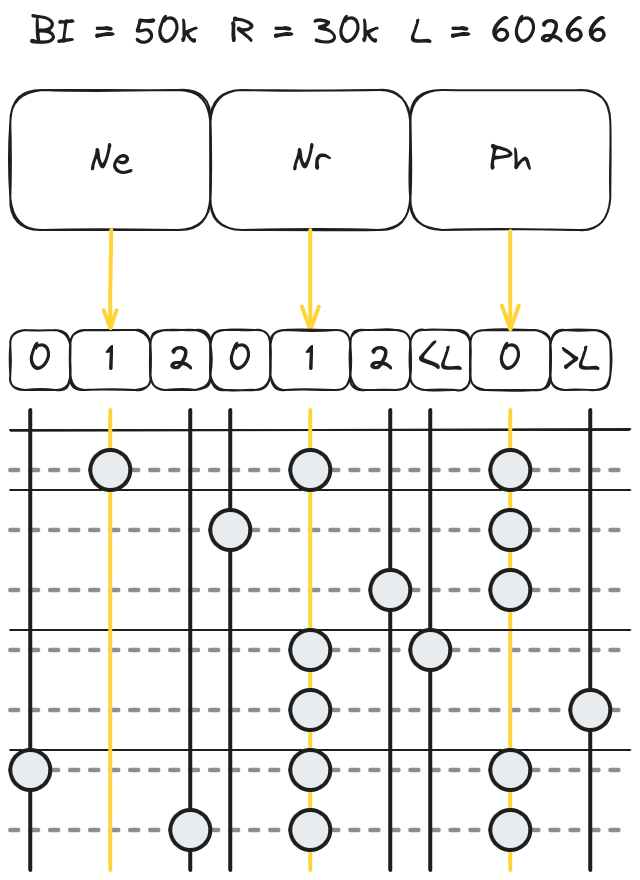
\includegraphics[width=0.5\textwidth]{arbol.png}
	\captionof{figure}{Árbol de decisiones \textit{base choice} con tres variables}
\end{minipage}

La mayoría de situaciones que resultan de la combinación de estas variables ya están
cubiertas por las pruebas de valores límite y clases de equivalencia realizadas anteriormente.
Este estudio demuestra, sin embargo, que se puede llegar a diseñar un sistema más complejo si
se desea alcanzar una mayor cobertura a costa de un gran número de situaciones ya cubiertas.
